% Figure 3: Fractal Antenna Structure (Sierpinski Triangle)
% Author: Dr. Computernonymouse
% Description: Sierpinski triangle fractal antenna for multi-scale ZPE coupling
%              showing self-similarity and fractal dimension

\documentclass[tikz,border=10pt]{standalone}
\usepackage{tikz}
\usepackage{pgfplots}
\usepackage{amsmath}
\usepackage{amssymb}
\usepackage{xcolor}

\pgfplotsset{compat=1.18}
\usetikzlibrary{calc,patterns,decorations.pathmorphing,backgrounds,shadings}

% Define metallic colors
\definecolor{metalsilver}{RGB}{168,168,168}
\definecolor{metaldark}{RGB}{105,105,105}
\definecolor{metallight}{RGB}{211,211,211}
\definecolor{substrate}{RGB}{255,248,220}
\definecolor{resonance1}{RGB}{255,127,14}
\definecolor{resonance2}{RGB}{44,160,44}
\definecolor{resonance3}{RGB}{31,119,180}

% Recursive Sierpinski triangle macro
\newcommand{\sierpinski}[2]{
    % #1 = recursion level, #2 = side length
    \ifnum#1=0
        \filldraw[metalsilver,draw=metaldark,line width=0.1pt]
            (0,0) -- (#2,0) -- ({#2/2},{#2*0.866}) -- cycle;
    \else
        \pgfmathtruncatemacro{\level}{#1-1}
        \pgfmathsetmacro{\half}{#2/2}
        \begin{scope}
            \sierpinski{\level}{\half}
        \end{scope}
        \begin{scope}[shift={(\half,0)}]
            \sierpinski{\level}{\half}
        \end{scope}
        \begin{scope}[shift={({0.25*#2},{0.433*#2})}]
            \sierpinski{\level}{\half}
        \end{scope}
    \fi
}

\begin{document}

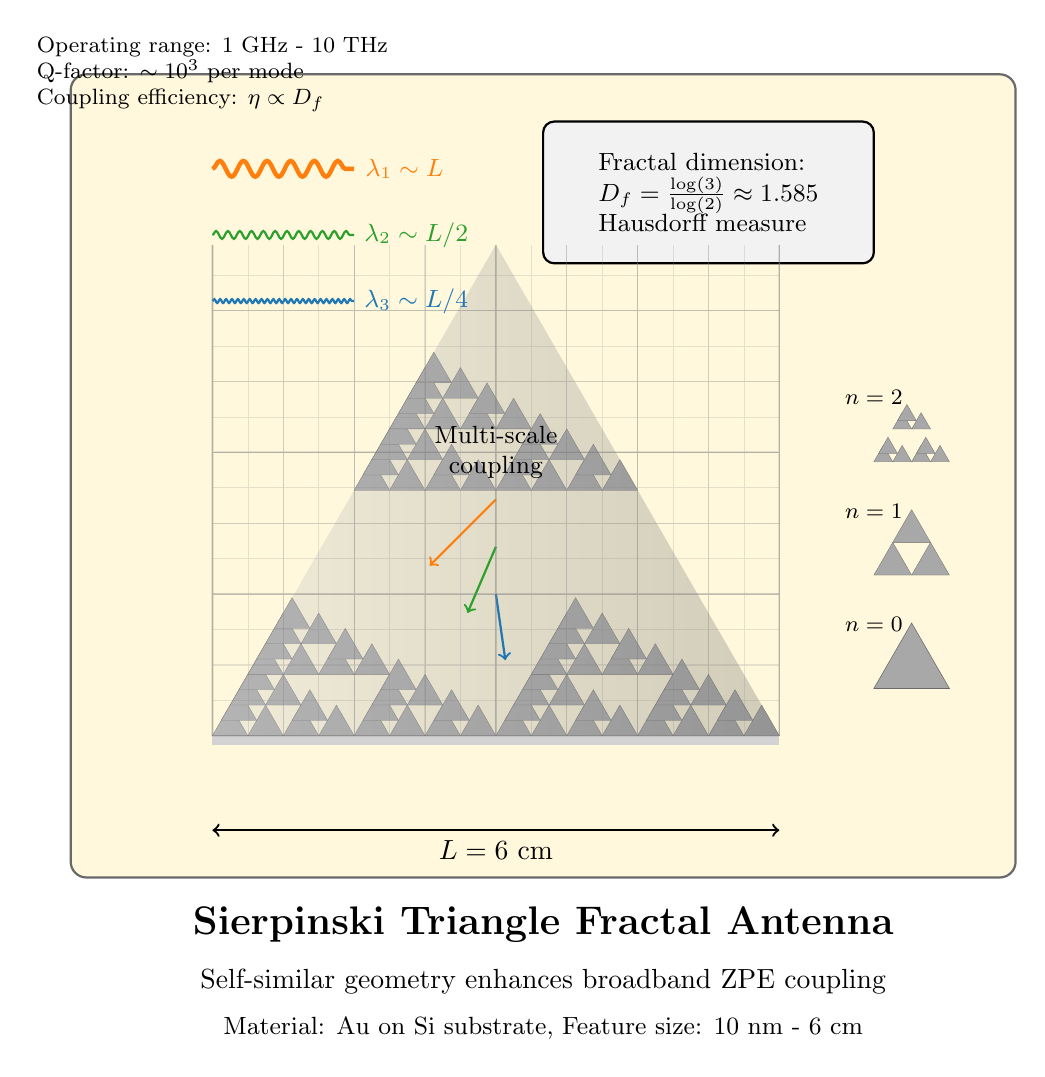
\begin{tikzpicture}[scale=1.2]

% Substrate background
\begin{scope}[on background layer]
    \fill[substrate,rounded corners=2mm] (-1,-1) rectangle (9,7.5);
    \draw[thick,metaldark,rounded corners=2mm] (-1,-1) rectangle (9,7.5);
\end{scope}

% Main Sierpinski triangle (4 iterations for detail)
\begin{scope}[shift={(0.5,0.5)}]
    % Metallic base plate
    \fill[metallight] (0,-0.1) rectangle (6,0);

    % Draw the Sierpinski fractal
    \sierpinski{4}{6}

    % Add metallic shading effect
    \begin{scope}[transparency group,opacity=0.3]
        \shade[left color=metallight,right color=metaldark]
            (0,0) -- (6,0) -- (3,5.196) -- cycle;
    \end{scope}
\end{scope}

% Scale indicators showing self-similarity
\begin{scope}[shift={(7.5,1)}]
    % Level 0 - single triangle
    \node[font=\footnotesize,above] at (0,0.5) {$n=0$};
    \filldraw[metalsilver,draw=metaldark,line width=0.2pt]
        (0,0) -- (0.8,0) -- (0.4,0.693) -- cycle;

    % Level 1
    \begin{scope}[shift={(0,1.2)}]
        \node[font=\footnotesize,above] at (0,0.5) {$n=1$};
        \sierpinski{1}{0.8}
    \end{scope}

    % Level 2
    \begin{scope}[shift={(0,2.4)}]
        \node[font=\footnotesize,above] at (0,0.5) {$n=2$};
        \sierpinski{2}{0.8}
    \end{scope}
\end{scope}

% Coupling frequency indicators (wavelike patterns)
\draw[resonance1,ultra thick,decorate,decoration={snake,amplitude=1mm,segment length=3mm}]
    (0.5,6.5) -- (2,6.5) node[right,font=\small] {$\lambda_1 \sim L$};

\draw[resonance2,thick,decorate,decoration={snake,amplitude=0.5mm,segment length=1.5mm}]
    (0.5,5.8) -- (2,5.8) node[right,font=\small] {$\lambda_2 \sim L/2$};

\draw[resonance3,thick,decorate,decoration={snake,amplitude=0.25mm,segment length=0.75mm}]
    (0.5,5.1) -- (2,5.1) node[right,font=\small] {$\lambda_3 \sim L/4$};

% Dimension and fractal annotations
\draw[<->,thick] (0.5,-0.5) -- (6.5,-0.5) node[midway,below] {$L = 6$ cm};

% Fractal dimension calculation box
\begin{scope}[shift={(4,5.5)}]
    \draw[thick,rounded corners,fill=white!90!gray]
        (0,0) rectangle (3.5,1.5);
    \node[align=left,font=\small] at (1.75,0.75) {
        Fractal dimension:\\
        $D_f = \frac{\log(3)}{\log(2)} \approx 1.585$\\
        Hausdorff measure
    };
\end{scope}

% Multi-scale coupling annotation
\draw[->,thick,resonance1] (3.5,3) -- (2.8,2.3);
\draw[->,thick,resonance2] (3.5,2.5) -- (3.2,1.8);
\draw[->,thick,resonance3] (3.5,2) -- (3.6,1.3);
\node[align=center,font=\small] at (3.5,3.5) {Multi-scale\\coupling};

% Title and technical specs
\node[font=\Large\bfseries] at (4,-1.5) {Sierpinski Triangle Fractal Antenna};
\node[font=\normalsize] at (4,-2.1) {Self-similar geometry enhances broadband ZPE coupling};
\node[font=\small] at (4,-2.6) {Material: Au on Si substrate, Feature size: 10 nm - 6 cm};

% Grid overlay showing scale invariance
\begin{scope}[shift={(0.5,0.5)},opacity=0.2]
    \draw[step=0.375,gray,very thin] (0,0) grid (6,5.196);
    \draw[step=0.75,gray,thin] (0,0) grid (6,5.196);
    \draw[step=1.5,gray] (0,0) grid (6,5.196);
    \draw[step=3,gray,thick] (0,0) grid (6,5.196);
\end{scope}

% Technical parameters box
\begin{scope}[shift={(0.5,7.5)}]
    \node[align=left,font=\footnotesize] at (0,0) {
        Operating range: 1 GHz - 10 THz\\
        Q-factor: $\sim 10^3$ per mode\\
        Coupling efficiency: $\eta \propto D_f$
    };
\end{scope}

\end{tikzpicture}

\end{document}